\chapter{はじめに}
\label {chp:tex_basic}

\section{研究の背景と目的}
\label{sec:tex_basic_section}
昨今,コロナの影響により,人と直接会う機会が減り,マスクの着用を強いられるようになった.
その結果,笑顔になる機会が減るため,笑顔の減少に繋がる.
しかし,総合人材サービスのパーソルホールディングス株式会社が行った調査[1]では,
仕事をする上で笑顔になると「楽しい」という気持ちが高まった人は約6割で,
ポジティブな感情状態で仕事に取り組んでいた人ほど,笑顔になっており,
職場において笑顔が高まれば,自発的に取り組む傾向があるという結果が出た.

\begin{figure}[!h]
    \begin{center}
        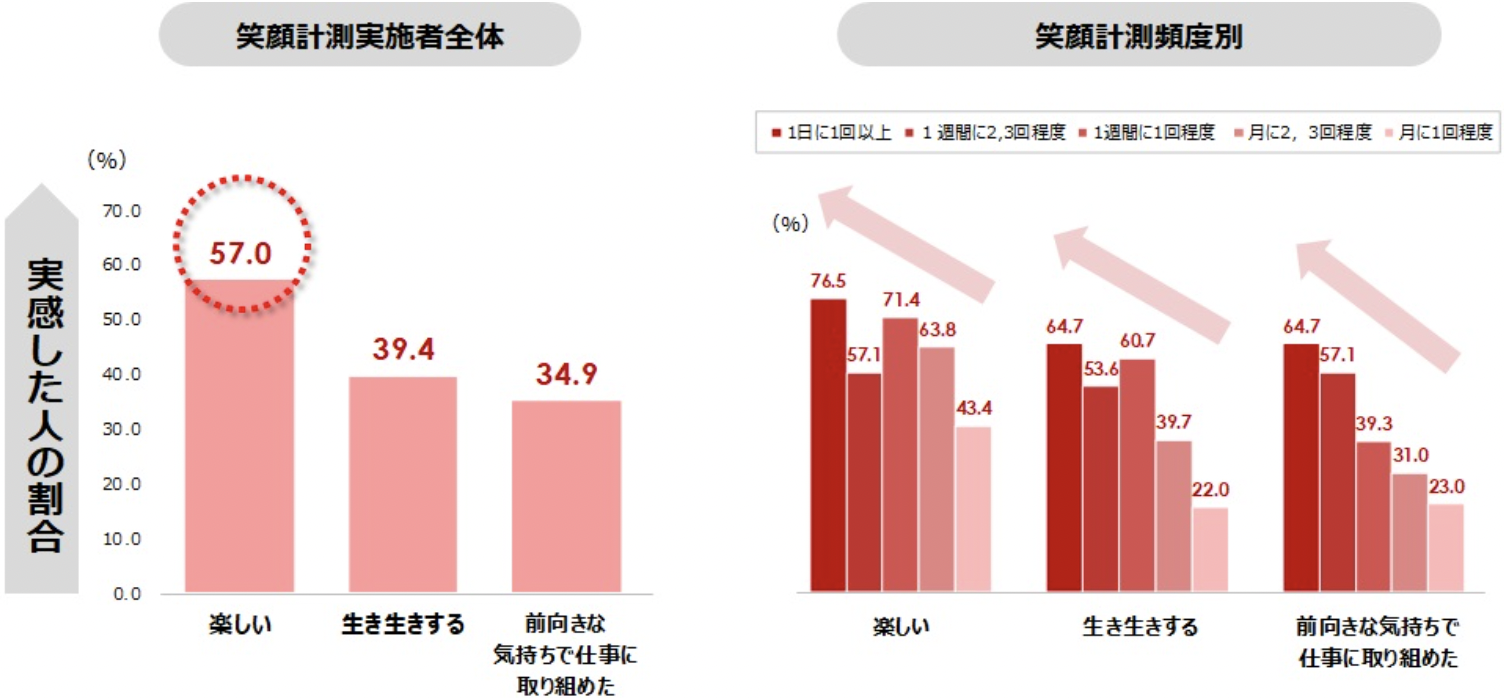
\includegraphics[scale=0.5, clip]{./img/work.png}
        \caption{笑顔計測後の主な感情変化}
        \label{fig:図の名前}
    \end{center}
\end{figure}

また,厚生労働省の調査[2]によると,下のグラフから分かるように,厚生労働省の調査によると,
平成19年度から令和元年にかけて約15\%も増加している.

\begin{figure}[!h]
    \begin{center}
        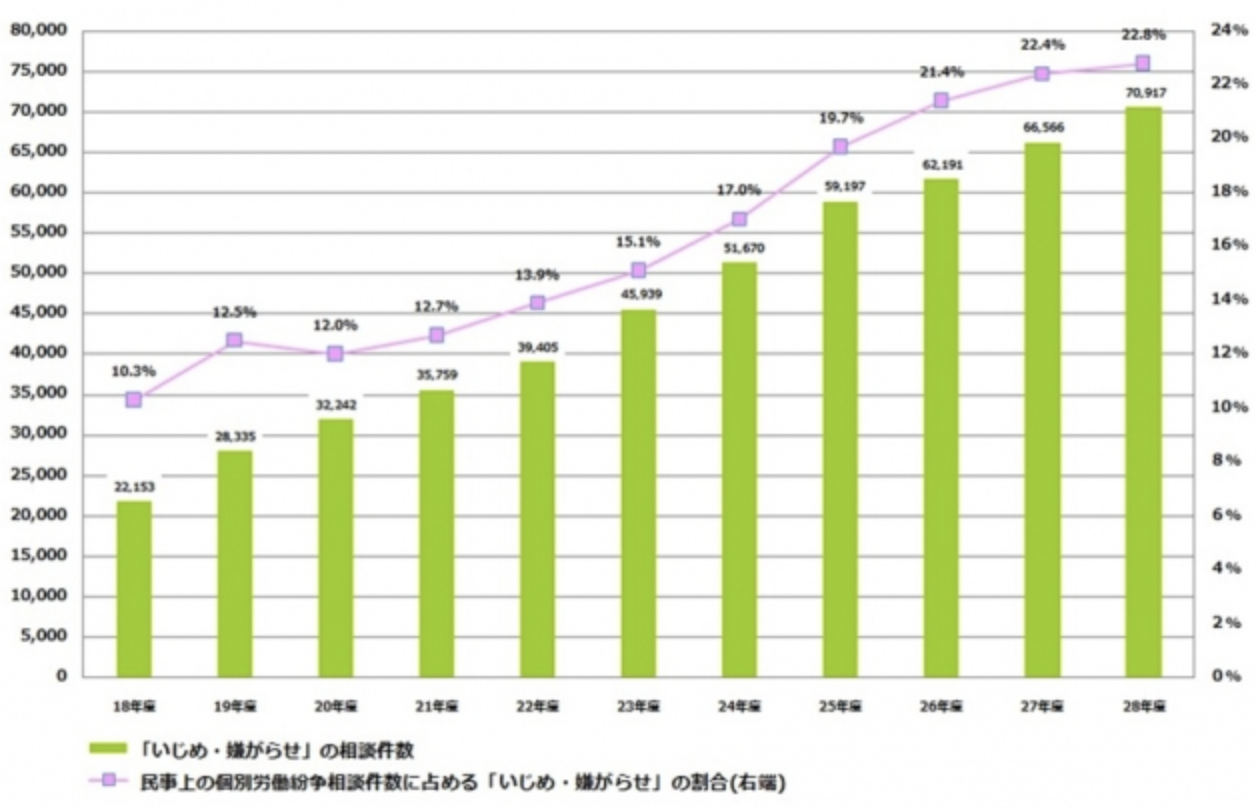
\includegraphics[scale=0.6, clip]{./img/graph.png}
        \caption{厚生労働省によるパワハラ調査}
        \label{fig:図の名前}
    \end{center}
\end{figure}

そこで我々は,以上の課題である「笑顔の減少」と「パワハラの増加」の解決を目的に
FaceAPIを用いた表情分析を活用した労務管理支援システムを提案する.

\vspace{8mm}

\section{論文の構成}
\label{sec:tex_basic_newline}
    改行は\verb|\\|というように,バックスラッシュ(円マーク)を続けて二つ記述します.\\
    \%を書くと以降がコメントアウトされます.

    エディタ上で一行空白をあけて記述することで,新たな文節として認識されます.

\section{環境とコマンド}
\label{sec:tex_basic_envcmd}
    Latexには「環境」と「コマンド」があります.
    環境は複数行にまたがるもので,コマンドは一行のみ有効なものです.
\subsection{環境}
\label{sub:tex_basic_section_envcmd_env}
    環境を使用するときは\verb|\begin{環境名}と\end{環境名}|で囲みます.\\
    画像を表示,表を作成,箇条書き等さまざまな場面で使用します.
\subsection{コマンド}
\label{sub:tex_basic_section_envcmd_cmd}
    コマンドは\verb|\newpage|のように先頭に\verb|\|をつけた単語を記述します.\\
    環境と同様にさまざまな種類があります.

\section{エスケープ}
\label{sec:tex_basic_escape}
    \# \$ \& \% \{ \}  \\
    などがエスケープの必要な文字です.直前に\verb|\|をつけるとエスケープされます.\\
    文章全体をエスケープする場合は「verbatim」環境を使用します.
     
\section{箇条書き}
\label{sec:tex_basic_clause}
    箇条書きを行う場合にはitemize環境を使用します.\\
    改行を入れることで題目と説明のように表示することが可能です.\\
    |記述例|\\
    \verb|\begin{itemize}|\\
        \verb|\item| あいてむ1\\
        \verb|\item| あいてむ2\\\\
        あいてむ2について\\
    \verb|\end{itemize}|\\\\
    |表示例|
\begin{itemize}
    \item あいてむ1
    \item あいてむ2

    あいてむ2についてあいてむ2についてあいてむ2についてあいてむ2についてあいてむ2についてあいてむ2についてあいてむ2についてあいてむ2についてあいてむ2についてあいてむ2についてあいてむ2についてあいてむ2についてあいてむ2についてあいてむ2についてあいてむ2について
\end{itemize} 

    箇条書きには複数種類があります.\\
    itemize環境の場合は通常の「・」,enumerate環境の場合は「1.」のように数字列挙に,description環境の場合は「\verb|\item[項目A] 説明文|」と書くことで項目つきの箇条になります.